\section{Visualization}
\nblink{brats/13\_testnet\_hausdorff\_masks.ipynb}
\nblink{brats/14\_brats\_hausdorff\_masks.ipynb}

doc: grafiken von HDM sehen teilweise gleich aus => sind sie nicht, skalierungsproblem


raw, absolute, worse, better

\begin{figure}[H]
    \centering
    \begin{subfigure}{.33\textwidth}
        \centering
        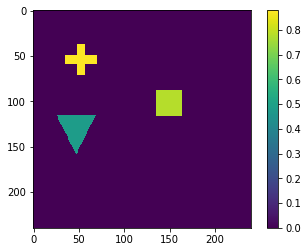
\includegraphics[width=\linewidth]{chapters/06_hdm/visualization/original.png}
        \caption{TODO}
    \end{subfigure}%
    \begin{subfigure}{.33\textwidth}
        \centering
        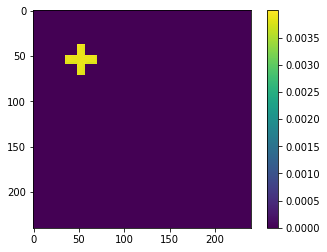
\includegraphics[width=\linewidth]{chapters/06_hdm/visualization/ground_truth.png}
        \caption{TODO}
    \end{subfigure}
        \begin{subfigure}{.33\textwidth}
        \centering
        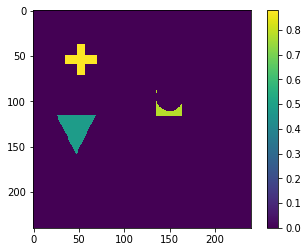
\includegraphics[width=\linewidth]{chapters/06_hdm/visualization/masked.png}
        \caption{TODO}
    \end{subfigure}
    \caption{TODO}
\end{figure}

\begin{figure}[H]
    \centering
    \begin{subfigure}{.5\textwidth}
        \centering
        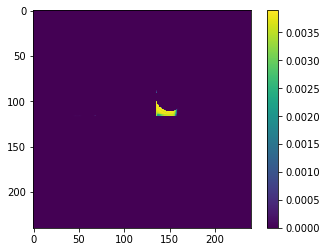
\includegraphics[width=\linewidth]{chapters/06_hdm/visualization/segment.png}
        \caption{Original shape}
    \end{subfigure}%
    \begin{subfigure}{.5\textwidth}
        \centering
        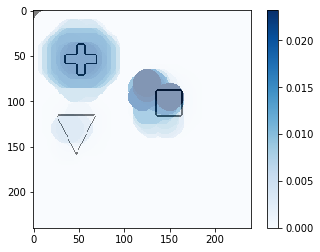
\includegraphics[width=\linewidth]{chapters/06_hdm/visualization/hdm_raw.png}
        \caption{Shape moved to the right}
    \end{subfigure}
    \caption{Hausdorff distance between the left and the right figure: 1353. }
    \label{hdm_smaller_circles}
\end{figure}


\begin{figure}[H]
    \centering
    \begin{subfigure}{.5\textwidth}
        \centering
        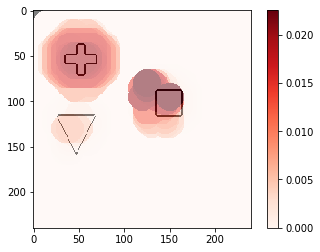
\includegraphics[width=\linewidth]{chapters/06_hdm/visualization/hdm_worse.png}
        \caption{Original shape}
    \end{subfigure}%
    \begin{subfigure}{.5\textwidth}
        \centering
        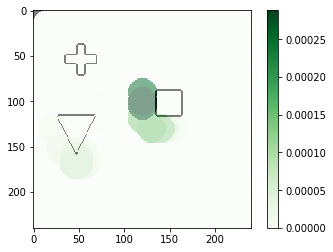
\includegraphics[width=\linewidth]{chapters/06_hdm/visualization/hdm_better.png}
        \caption{Shape moved to the right}
    \end{subfigure}
    \caption{Hausdorff distance between the left and the right figure: 1353. }
    \label{hdm_smaller_circles}
\end{figure}
